\chapter{Revisão Bibliográfica}\label{RevisãoBibliográfica}

Neste capítulo, é apresentada a revisão bibliográfica deste trabalho. Esta abrange os principais temas abordados: Sensores Inerciais(IMU), Orientação de Objetos, Detecção de Manobras automotivas.

\section{Navegação}
De acordo com \citeauthor*{grewal2007global} existem 5 formas basicas de navegação, sendo elas:
\begin{enumerate}
    \item \textbf{Pilotagem} - Que consiste no reconhecimento do ambiente de forma a dizer onde se está
    \item \textbf{\textit{Dead Reckoning}}, que implica em saber de onde se partiu o movimento, mais alguma forma de estimativa de direção e velocidade
    \item \textbf{Navegação Celestial}, que utiliza o tempo e angulo entre o vertical local e objetos celestias conhecidos
    \item \textbf{Navegação por rádio}, que se baseia, em fontes de frequências de rádio com posições conhecidas
    \item \textbf{Navegação Inercial}, que se baseia no conhecimento prévio da posição velocidade e orientação mantendo-as ao longo do percurso a partir de medições de aceleração e direções espaciais conhecidas por meio de instrumentos que mecanizam as leis do movimento de Newton
\end{enumerate}{}

Dadas as formas de navegação outro conceito abordado são os sistema de navegação que são utilizados para se obter determinações automáticas da posição e velocidade de um objeto. Tem-se que um sistema de navegação pode ser dependente (ex.: navegação por rádio) ou não (ex.: Sistemas de navegação inercial - INS) de infraestrutura externa. A saída, ou resultado, de um sistema de navegação é conhecido como Solução de Navegação \cite{groves2008principles}

Assim sendo, o conceito de navegação possui como requisito primordial o posicionamento, que por sua vez é dependente do referencial ou de um sistema de referenciais. 

\section{Navegação Inercial}

Da mecânica básica, tem-se que a inércia é a tendência de um corpo em permanecer em repouso ou em movimento retilíneo uniforme desde que não haja nenhuma influência de forças externas.

Um sistema de coordendas inercial, nada mais é, que um sistema de coordenadas onde as leis newtonianas da física são validas. Dessa forma, sistemas de coordenadas inercias não estão rotacionando ou acelerando \citep{groves2008principles}.

De acordo com \citeauthor{groves2008principles} Os sistemas inerciais de navegação consistem em:
Primeiramente, uma unidade de medida inercial (IMU) contendo um agrupamento de sensores, que são montados sob uma base comum de modo a manter a mesma orientação relativa. Segundamente em computadores de navegação que processam as grandezas inerciais.



\section{Sensores Inerciais(IMU)}

Os sensores inerciais mensuram o movimento linear e/ou angular pelo processamento de grandezas de um ou mais sensores inerciais. Tais sensores são usualmente, acelerômetros e giroscópios.

Os giroscópios fornecem medidas da mudança de atitude de um objeto ou sua taxa de rotação, em relação a um espaço inercial.
Acelerômetros, por sua vez, fornecem uma medida da força por unidade de massa exercida no sensor. Na prática, os acelerômetros não são capazes de separar a aceleracão total do objeto da aceleração devida a presença do campo gravitacional. Em vista disso, as medidas fornecidas pelos acelerômetros, quando em presença de um corpo massivo como a terra, devem ser combinadas com o conhecimento prévio do campo gravitacional, a fim de se determinar a aceleração do objeto com respeito ao espaço inercial \cite{groves2008principles}.

Lançando-se mão das medições de rotação, e das forças aplicadas no objeto é possivel, então, estimar velocidade, orientação e posição em relação a um determinado sistema de referência.

A maior parte dos tipos de acelerômetros e giroscópios realizam medições em um único eixo. Uma IMU combina, em geral três sensores de cada, de forma a produzir uma medição tridimensional de aceleração e velocidade angular (\citeauthor{groves2008principles},\citeyear{groves2008principles})

Outro sensor muito presente em IMU é o magnetômetro que consiste em um sensor capaz de medir a densidade do fluxo magnético. Este possui como principal função na navegação fornecer uma referência em direção ao norte geográfico.

\section{Sistemas de Coordenadas}

\citeauthor*{kovalevsky2012reference}(\citeyear{kovalevsky2012reference}), afirma que movimento e posição não são conceitos absolutos, portanto, podem ser descritos apenas em relação a um referencial.

Em termos de um problema de mecânica simples, a modelagem do movimento é feita em relação ao referencial terrestre, que neste caso, é considerado um referencial inercial. Assumir isto é razoável visto que simplifica o desenvolvimento de soluções. No entanto \citeauthor{mori2013uso} afirma que na navegação, esta premissa não se aplica. Visto que, a rotação da terra impacta significantemente nos cálculos de navegação, principalmente com relação a grandes distâncias.

Outra problemática, diz respeito aos diferentes referenciais inerciais envolvidos em um problema de navegação. Ressalta-se que Os sensores inerciais medem o movimento em relação ao referencial, o GPS, por exemplo, será responsável por fornecer a posição e velocidade de uma antena de um receptor em relação a uma constelação de satélites. Por fim o usuário do sistema, deseja saber a sua posição em relação a Terra. 

Fica claro que para uma navegação acurada, a relação entre esses diversos sistemas de coordenadas deve ser modelada de forma correta.

A definição de um sistema de coordenadas pode se dar de duas maneiras\citep{groves2008principles}:

\begin{enumerate}
    \item Através da definição de uma origem e um conjunto de eixos nos quais o movimento de um objeto pode ser descrito
    \item através da definição da posição e orientação de um determinado objeto
\end{enumerate}{}

Um sistema de referencial ortogonal possui seis graus de liberdade, a posição de origem e a orientação dos eixos ($x, y$ e $z$). Estes, por sua vez, devem ser expressos em relação a outro sistema a fim de defini-los. De acordo com \citeauthor{groves2008principles} (\citeyear{groves2008principles}) qualquer problema de navegação deve envolver dois sistema de coordenadas: Um sistema do objeto e um sistema de referência. O sistema do objeto descreve o corpo cuja posição e/ou orientação se quer obter (ex.: Celular). O sistema de referência descreve um corpo conhecido (ex.: Terra, Carro) relativo ao qual a posição e/ou orientação é desejada.

\section{Referencias de Navegação}

Nesta secção serão apresentados alguns referências comumente utilizados em navegação.

\subsection{Referencial ECI(Earth Centered Inertial)}

Se trata de um sistema nominalmente centrado no centro de massa da terra e orientado em relação ao seu eixo de rotação. Assim sendo, esse referencial possui uma aplicação mais teórica do que prática \citep{mori2013uso}, uma vez que terra não pode ser considerada um referencial inercial por definição.

\subsection{Referencial ECEF(Earth-Centered Earth-Fixed)}

Consiste no referencial similar ao ECI, no entanto, os seus eixos são paralelos em relação a Terra e acompanham durante o movimento. Neste caso, o eixo $z$ aponta na direção de rotação da Terra, de seu centro(origem), até o polo norte (verdadeiro); o eixo $x$ aponta para o centro da intersecção do equador com o meridiano de referência, que define a longitude $0\deg$; o eixo $y$ completa o sistema (regra da mão direita)

\subsection{Referencial de Navegação Local NED (North-East-Down)}

É utilizado amplamente em navegação \citep{mori2013uso}. Trata-se de um referencial que representa a Terra como uma superfície plana. A origem, nesse caso, se dá pelo ponto onde a solução de navegação foi configurada(ex.: centro de massa do veículo). O eixo $z$ é definido pela Normal ao elipsoide de referência; $x$, nesse caso, aponta em direção ao pólo norte; $y$ aponta em direção ao leste. Dispositivos móveis em geral, quando possuem o magnetômetro, possuem a opção de transformar o eixo de coordenadas local, neste sistema de referência.

\begin{figure}
    \centering
    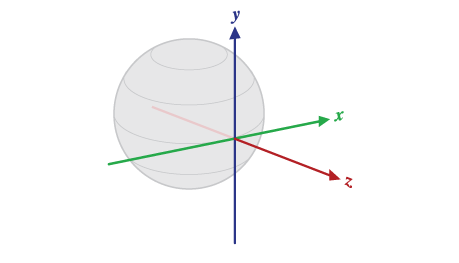
\includegraphics{Figuras/referencialterra.png}
    \caption{Referencia NED \\ Fonte: Documentação Android}
    \label{fig:referencialTerra}
\end{figure}{}

\subsection{Referencial do Veículo (Body Frame)}

Este referencial está fixo ao corpo e compreende a origem e orientação do objeto para qual a solução de navegação é utilizada. Assim sendo, a origem coincide com a origem do referencial local, no entanto os eixos são fixos em relação ao veículo. O eixo $z$ é normal ao solo; $y$ possui a mesma direção do movimento e $x$ completa o conjunto ortogonal.
Em termos do movimento angular: $z$ é o eixo de \textit{yaw}; $y$ o eixo de \textit{roll} e $x$ o eixo de \textit{pitch}

\section{Transferência de Coordenadas}

Dados dois referenciais inerciais

\begin{figure}
    \centering
    \subfloat[Vetores Alinhados.]{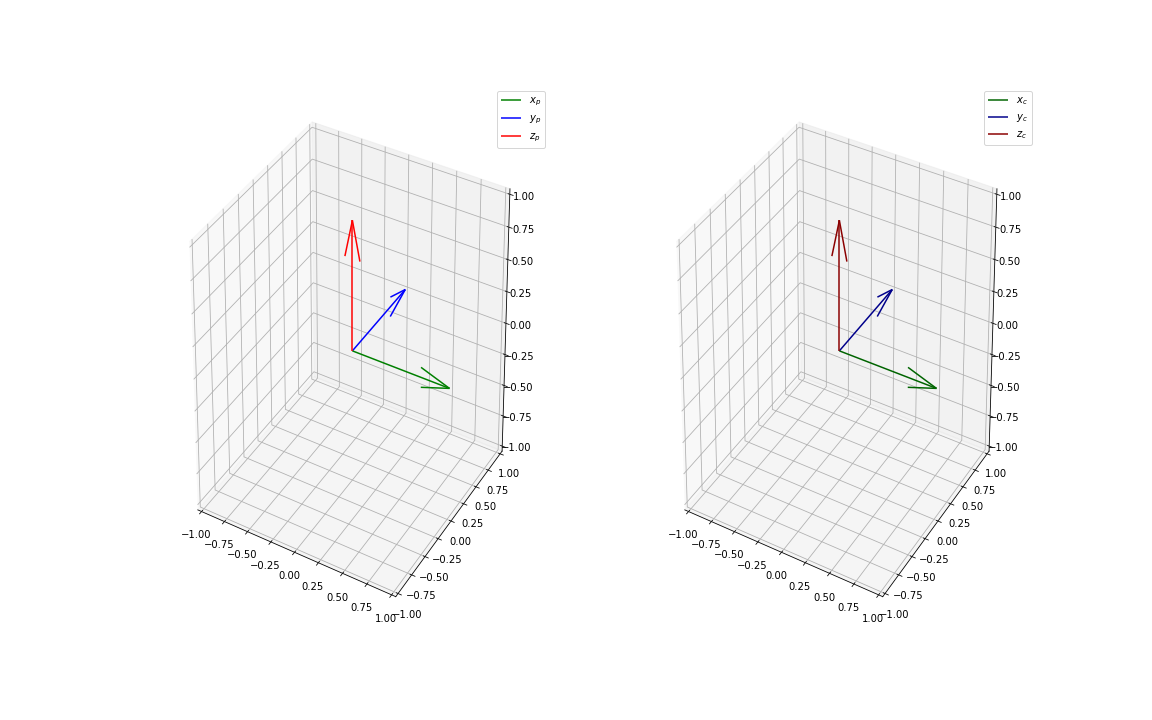
\includegraphics[height=70mm,width=\textwidth]{Figuras/alinhamentoDeVetores1.png}}
    \\
    \subfloat[Vetores com Eixos Invertidos.]{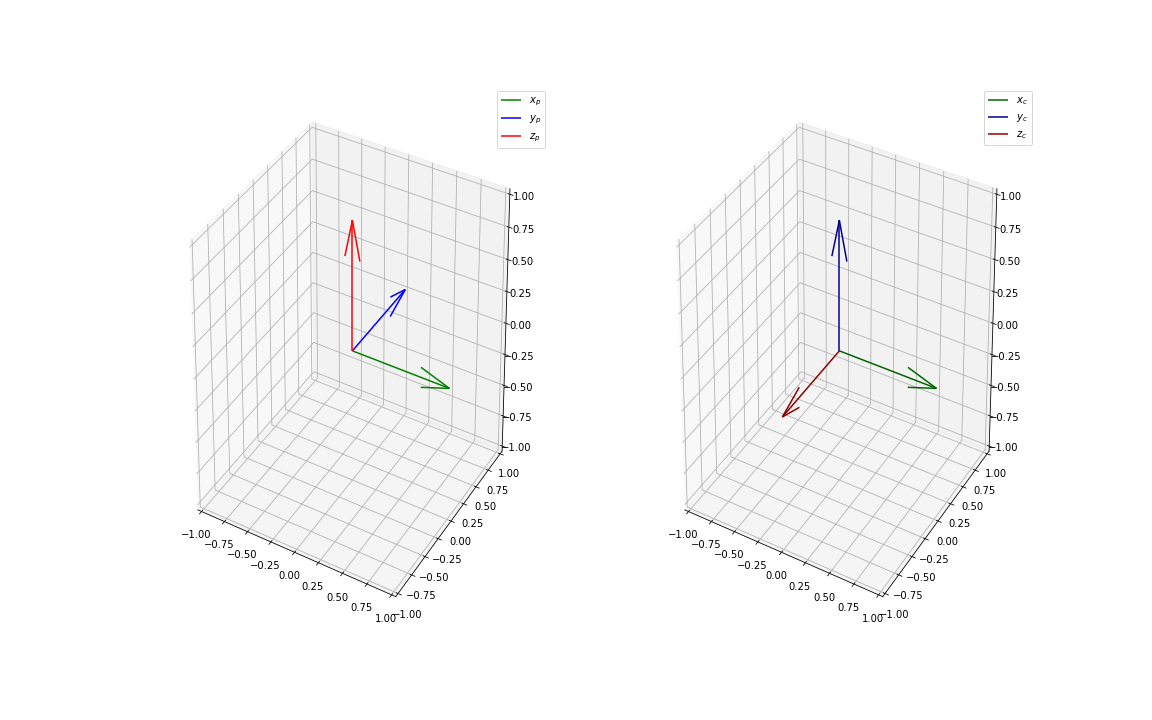
\includegraphics[height=70mm,width=\textwidth]{Figuras/alinhamentoDeVetores2.png}}
    \\
    \subfloat[Vetores caso Genérico.]{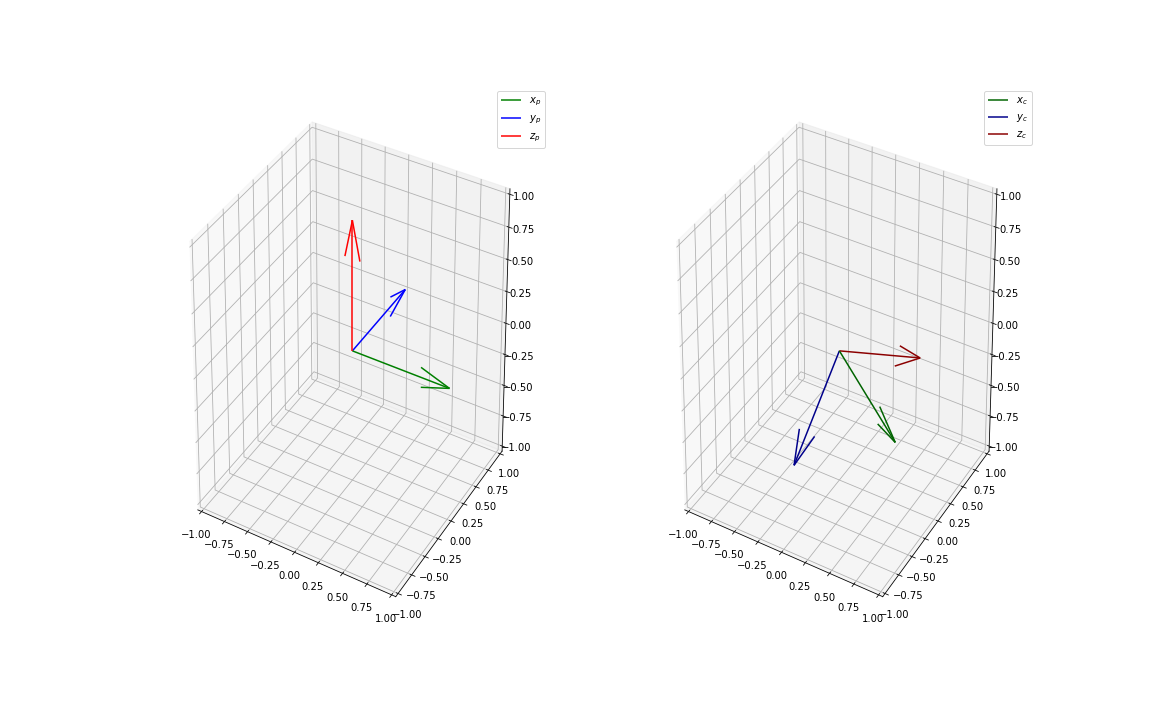
\includegraphics[height=70mm,width=\textwidth]{Figuras/alinhamentoDeVetores3.png}}
    \caption{Alinhamento de Vetores}
    \label{fig:alinhamentoDeVetores}
\end{figure}{}

\begin{equation} 
A_c = 
    \begin{bmatrix}
X_c\\ 
Y_c\\ 
Z_c
\end{bmatrix} e, A_p = 
    \begin{bmatrix}
X_p\\ 
Y_p\\ 
Z_p
\end{bmatrix}
\end{equation}{}

a transformação da base entre eles se dá por meio de uma matriz da forma:
\begin{equation}
    A_c = T . A_p
    \label{eq:equaçaoDaRotacao}
\end{equation}{}

onde:
\begin{equation}
    T = \begin{bmatrix}
T_{x_i} & T_{x_j}  & T_{x_k} \\ 
T_{y_i} & T_{y_j}  & T_{y_k} \\ 
T_{z_i} & T_{z_j}  & T_{z_k}
\end{bmatrix}
\end{equation}{}

Observando a Figura \ref{fig:alinhamentoDeVetores}(a) fica claro que a matriz de rotação nesse caso é a Identidade. Tal relação é tipicamente relevante quando se aborda o problema da transformação de base de um celular dentro de um veículo. Visto que, tomando a base $A_c$, como o sistema de coordenadas do carro. $y$ representaria movimentos de aceleração e desaceleração do veículo (aceleração longitudinal), $x$ representaria acelerações laterais e $z$ elevações. Tal percepção permite derivarmos a matriz de rotação para qualquer posição dentro de um veículo contanto que saibamos as direção da aceleração para frente e a gravidade. Como por exemplo no caso da Figura \ref{fig:alinhamentoDeVetores}(b) onde a matriz de rotação é :

\begin{equation}
    T = \begin{bmatrix}
1 & 0  & 0 \\ 
0 & 0  & -1 \\ 
0 & 1  & 0
\end{bmatrix}
\end{equation}{}

que aplicando na Equação \ref{eq:equaçaoDaRotacao} para esse caso em específico tem-se:

\begin{equation}
\begin{bmatrix}
1 & 0  & 0 \\ 
0 & 1  & 0 \\ 
0 & 0  & 1
\end{bmatrix} = 
\begin{bmatrix}
1 & 0  & 0 \\ 
0 & 0  & -1 \\ 
0 & 1  & 0
\end{bmatrix}
\begin{bmatrix}
1 & 0  & 0 \\ 
0 & 0  & 1 \\ 
0 & -1  & 0
\end{bmatrix}
\end{equation}{}


De modo que $T_{\hat{i}}$ representa a aceleração lateral sentida pelo celular, $T_{\hat{j}}$ representa a aceleração longitudinal, e $T_{\hat{k}}$ representa a Normal.
A partir disso, é possível se gerar uma matriz de rotação para uma posição genérica do celular contanto que se saiba a direção das acelerações.




\section{Orientação do Veículo}
A forma mais comum de estimar a orientação de um veículo é se utilizando de um sistema global de navegação por satélite (GNSS)\cite{almazan2013full}, como o GPS, por exemplo. 

A direção do carro pode ser medida através de dois GPS(frontal e traseiro) ou calculando-se a diferença entre dois pontos consecutivos. A priori, esse método de posicionamento possui diversas limitações: A frequência máxima é aproximadamente 1 $Hz$; isso significa que a 60 $Km/h$, um veículo teria se deslocado 20m da sua posição inicial. Ainda devido a baixa frequência, não se é possível captar movimentos bruscos em uma viagem comum de carro, que ocorrem em frações de segundos. Ressalta-se \cite{almazan2013full} que esse tipo de monitoramento não funcionam sob baixa visibilidade de satélites (tuneis e viadutos em geral).

Li \cite{li2009vehicle} utilizou a fusão de sensores, baseada em um sistema de observador de cascata e foi capaz de estimar a direção e velocidade do veículo inclusive durante manobras complexas, com elevada acurácia. Tendo-se em vista que informações como o angulo do volante, e a pressão realizada nos pedais do veículo são diretamente relacionados com o dinâmica do sistema. 

Com o proposito de lançar mão desse tipo de informação a respeito do veículo (que é transmitida através do protocolo bus-CAN) diversas pesquisas utilizam um conector OBD-II de forma a coletar os dados. A grande vantagem desse método consiste em aumentar em atingir uma frequência mais de 1 $Hz$ não limitada ao campo aberto para estimar o estado do veículo. No entanto existem duas contra-indicações. Primeiramente, se trata de um método invasivo que obriga o usuário a plugar um novo dispositivo no veículo. Segundamente, cada fabricante de veículo possui seu próprio protocolo \cite{almazan2013full} e todos deveriam ser conhecidos previamente para arquitetar uma solução barata e genérica.

Assim sendo, um método adotado para medir a dinâmica veicular, têm sido o uso de dispositivos portáteis, que se utilizam de uma combinação da medição do campo magnético da terra (através de um magnetômetro) e um outro sensor, como o GPS ou algum sensor inercial.
Existem alguns trabalhos (\citep{zheng2016unsupervised}, \citep{zheng2015mobileutdrive},\citep{almazan2013full}) na literatura que utilizam-se dessa combinação para se estimar a orientação de um smartfone no interior de um veículo. A vantagem desse método advém do aumento da frequência de captura de dados. Porém é um método significantemente influenciado por interferência de campos magnéticos \cite{almazan2013full}. Nesse sentido, a sensibilidade do magnetômetro é alta e devido a grande quantidade de componentes eletro-mecânicos no veículo, seu comportamento é altamente comprometido. 

Além disso, existem trabalhos que buscam utilizar a fusão de sensores inerciais (IMU) e GNSS para superar as limitações já mencionadas a respeito dos GNSS. Todavia, a orientação de um IMU no veículo deve ser conhecida anteriormente, de forma a se obter medições condizentes com a dinâmica do veículo.

Em linhas gerais, é necessário saber a posição do smartfone em relação ao sistema de coordenadas do veículo para que se possa combinar os sensores inerciais com o GNSS.

\citet{you2013carsafe} Propôs um aplicativo que visa alertar o motorista desatento, através da utilização de duas câmeras. \citeauthor*{bergasa2014drivesafe}\citep{bergasa2014drivesafe} propuseram um aplicativo que também possui como objetivo alertar desatenção e pontuar o motorista utilizando visão computacional, em conjunto com sensores IMU do smartfone, GPS e o microfone do aparelho. Em ambos os casos os autores se utilizam do aparelho fixo de forma a realizar a fusão de sensores. A solução proposta por esses autores, busca imitar algumas funcionalidades encontradas em diversos veículos top de linha no mercado. Ainda assim se apresentando como uma alternativa as "caixas-pretas" fornecidas, muitas das vezes, por seguradoras.

\citeauthor{chen2015d} argumenta em seu trabalho que ao monitorar o comportamento anormal de direção é possível conscientizar o motorista dos seus próprios hábitos. Uma vez que grande parte dos motoristas são autoconfiantes e não estão cientes de seus comportamentos agressivos. Ao identificar os hábitos ruins de direção automaticamente, o motorista pode tornar-se consciente de seu comportamento e então corrigi-lo. Assim podendo evitar futuros acidentes em potencial. Com isso em vista, \citeauthor{chen2015d} foi capaz de usar SVM para detectar 6 manobras de direções, a partir de 16 características extraídas com base em 6 meses de corridas coletadas. Todas as viagens foram realizadas com o celular alinhado com o carro.

\citeauthor{eren2012estimating} por sua vez foi capaz de classificar estilos de direção utilizando IMU e dados de GPS. Através de um algortimo de DTW, para compensar as diferenças temporais dos eventos. Da mesma forma que \citeauthor{fazeen2012safe} contribuiu com um sistema de monitoramento do comportamento do motorista que o avisa na ocorrência de manobras perigosas. Entretanto ambos os sistemas dependem do alinhamento do smartfone com o veículo, de modo a extrair as informações corretas dos sensores.

Com o objetivo de alinhar o sistema de coordenadas do aparelho celular com o carro \citeauthor*{dai2010mobile}\citep{dai2010mobile} sugeriram uma calibração baseada em IMU para obter os ângulos de "\textit{roll}" e "\textit{pitch}" do smartfone. No entanto, foi assumido que o smartfone estava alinhado com o eixo longitudinal do veículo; ou seja o ângulo de "\textit{yaw}", nesse caso, deve ser nulo. De forma análoga \citeauthor{almazan2013full} propôs um método de auto-calibração que estima o ângulo de "\textit{yaw}" do smartfone, em relação ao veículo para o celular em uma posição genérica.

\citeauthor{castignani2015driver}, por outro lado, propôs um sistema \textit{fuzzy} para monitorar o comportamento do motorista onde a direção é classificada como calma ou agressiva. No estudo em questão, foi levada em consideração a magnitude do vetor aceleracão de forma a mitigar o problema de decompor a aceleração lateral e logitudinal.


 
\section{Detecção de Manobras}

\citeauthor{fazeen2012safe} Através do seu método de monitoramento proposto, estudou os padrões de direção utilizando um celular Nexus One em diversos cenários. Com isso ele foi capaz de demonstrar os padrões seguros e repentinos de diversas manobras. De acordo com Autor \citep{fazeen2012safe}, acelerações e desacelerações seguras nunca atingem uma força g maior que $\pm 0.3g $ (aproximadamente $3m/s^2$); já as manobras bruscas chegam a $\pm 0.5g$ (aproximadamente $5m/s^2$).

\citeauthor*{Paefgen:2012:DBA:2406367.2406412} de forma similar, foram capazes de criar uma aplicação mobile que avalia o comportamento do motorista com base em medições do acelerômetro que fornece de forma instantânea informações a respeito da qualidade da direção do motorista. De forma a buscar validação, eles compararam os eventos registrados pelo smartfone com os eventos medidos em um IMU fixo no veículo, em um estudo de campo controlado. Por fim os autores identificaram que os smartfones tendem a sobreestimar eventos críticos de direção.

Outra contribuição interessante partiu de \citeauthor{zheng2015mobileutdrive} (\citeyear{zheng2015mobileutdrive}) que mostrou que a velocidade angular observado no eixo $z$ de um dispositivo alinhado com o carro, possui elevada correlação com o ângulo do volante. 

